\section{Exécution \& tests} % (fold)
\label{sec:execution}

Pour ce projet, nous avons effectué des tests de validation sur les fonctions algébriques, afin de s'assurer que celles-ci marchaient correctement, et pouvoir plus facilement isoler les problèmes. De même, le code a été segmenté pour permettre une lecture plus aisée de l'ordre dans lequel s'effectuent les diverses opérations. Afin de facilité la mise en oeuvre de la factorisation par bloc, nous avons choisi de ne pas traiter les cas où la taille des blocs n'est pas multiple de la largeur et la longueur de la matrice.\\

Plusieurs fonctions intermédiaires ont été écrites afin de simplifier l'affichage, la génération ou encore la comparaison entre matrices (voir util.c et util.h).

Nous avons remarqué que pour des matrices de taille croissantes, des erreurs d'arrondis apparaissaient et se propagaient rapidement. Ainsi, pour des matrics de taille $30 \times 30$, les erreurs commençaient à être significatives dans le calcul du dtrsm (de l'ordre de $0.1$). Nous n'avons pas remarqué ce genre d'erreurs dans les autres algorithmes toutefois, excepté dgesv qui utilise directement deux dtrsm. 

\section{Performances} % (fold)
\label{sec:perf}

Une série de tests est lancée sur différentes tailles de matrice ou différents nombres de processus plusieurs fois, afin d'obtenir des temps d'exécution moyens. Nous avons remarqué que l'algorithme passait beaucoup de temps dans les fonctions de répartition des données sur les processus. Aussi avons-nous comparé les temps de calculs seulement. \\
La largeur des colonnes a été fixée à $64$, afin de pouvoir exécuter les calculs sur des matrices dont les tailles étaient des multiples de 2, pour simplifier la lecture des résultats. 
La Figure \ref{fig:sp-size} montre que plus les calculs sont importants, plus la parallélisation est effective.

\begin{figure}[H]
\centering
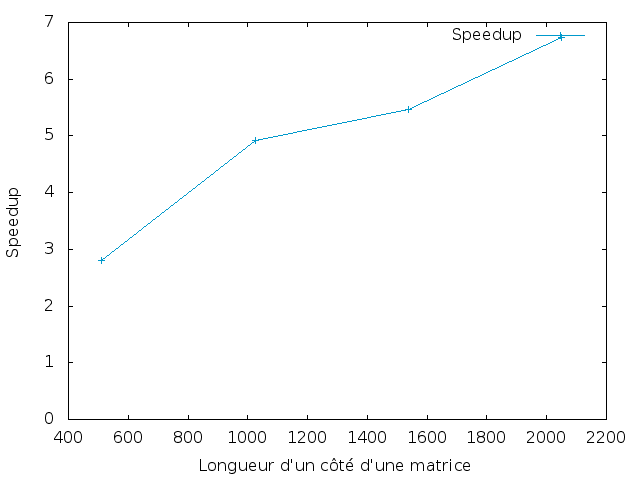
\includegraphics[width=0.8\textwidth]{sp-size.png}
\caption{Evolution du speedup avec la taille d'une matrice pour 8 processus}
\label{fig:sp-size}
\end{figure}

Comme l'indique la courbe de la Fig. \ref{fig:sp-proc}, le nombre de processeurs permet de réduire le temps d'exécution. Cette courbe a été tracée sur des matrices de dimensions $1024\times1024$. Nous pouvon remarquer que cette courbe est toujours inférieure à $y = x$. Le plateau ainsi que l'augmentation du speedup observés à 8 et 16 processus respectivement sont dus à la taille des blocs utilisé pour les colonnes (64 doubles de largeur dans l'exemple). Nous avons alors 2 colonnes à calculer par processus à partir de 8 processus et ce chiffre descend à 1 colonne par processus lorsque $64*16 = 1042$. Pour profiter d'une accélération avec plus de processus, il faudrait diminuer la taille de des blocs. Il est également possible de séparer les blocs colonne en plusieurs blocs pour augmenter le parallélisme, qui s'amenuise au fil de l'algorithme (il y a peu de communication et beaucoup de calculs).

\begin{figure}[H]
\centering
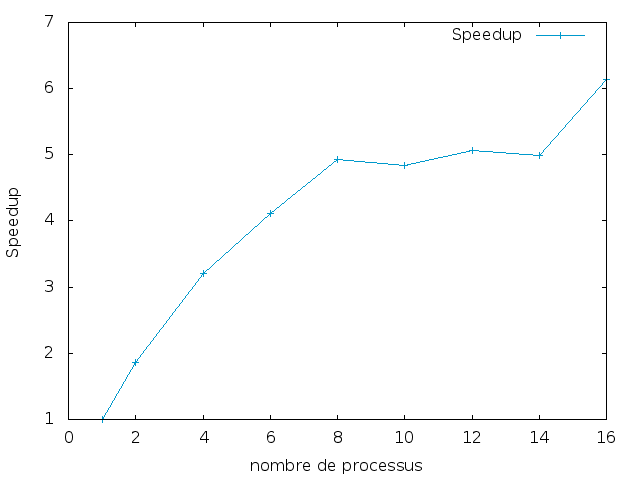
\includegraphics[width=0.8\textwidth]{sp-proc.png}
\caption{Accélération de notre programme par rapport au code séquentiel pour une matrice 1024x1024, en fonction du nombre de processeurs}
\label{fig:sp-proc}
\end{figure}

% section \ (end)
